% !TEX root = ../main.tex
In this section, we provide additional quantitative exploration of the upper bound studied in Section~\ref{sec:hierarchical_bayes}. 
The aim is to take steps towards relating the bounds to experimental results;
we know of little theoretical work in meta-learning that attempt to relate their results to
practical empirical datasets. Full details of the experiments in this section can be found in Appendix~\ref{app:exp_details}.

\subsection{Hierarchical Bayes polynomial regression}

We first focus on the setting of polynomial regression over inputs in the range $[-1,1]$. Some examples of these functions and samples are presented in Figure~\ref{fig:meta_lin_ref}, alongside the MAP and MLE estimates for the novel task. 

% We report the analytical expected risk, which is derived in Appendix~\ref{app:proofs:ubounds}, under different hyperparameter settings of the learning environment and varying sample sizes and task counts.

Figure~\ref{fig:hierarchical_lreg_simulation} shows the analytical expected error rate (risk) under various environment settings. We observe that even in this simple hierarchical model, the estimator exhibits complex behavior that is correctly predicted by Theorem~\ref{thm:lregression_bias_variance}. In Figure~\ref{fig:hierarchical_lreg_simulation}A, we varied the novel task difficulty by increasing the novel task observation noise ($\sigma^2_{M+1}$). We plot three curves for three different dataset size configurations. When the novel task is much noisier than the source tasks, it is greatly beneficial to add more meta-training data (blue vs. red). And while larger $k$ made little difference when the novel task was relatively difficult (blue vs. green), the expected loss was orders of magnitude lower when the novel task became easier. In Figure~\ref{fig:hierarchical_lreg_simulation}B, we fixed the relative task difficulty and instead varied $k$ and $M$. The x-axis now indicates the total data $Mn + k$ available to the learner. We observed that adding more tasks has a large effect in the low-data regime but, as predicted, the error has a non-zero asymptotic lower-bound --- eventually it is more beneficial to add more novel-task data samples.

These empirical simulations verify that our theoretical analysis is predictive of the behavior of this meta learning algorithm, as each of these observations can be inferred from Theorem~\ref{thm:lregression_bias_variance}. While this model is simple, it captures key features of and provides insight into the more general meta-learning problem. We also explored a non-linear sinusoid meta-regression problem \citep{finn2017model}, finding that our %linear 
theory is largely predictive of the general trends in this setting too.

\iflatexml
\begin{figure}
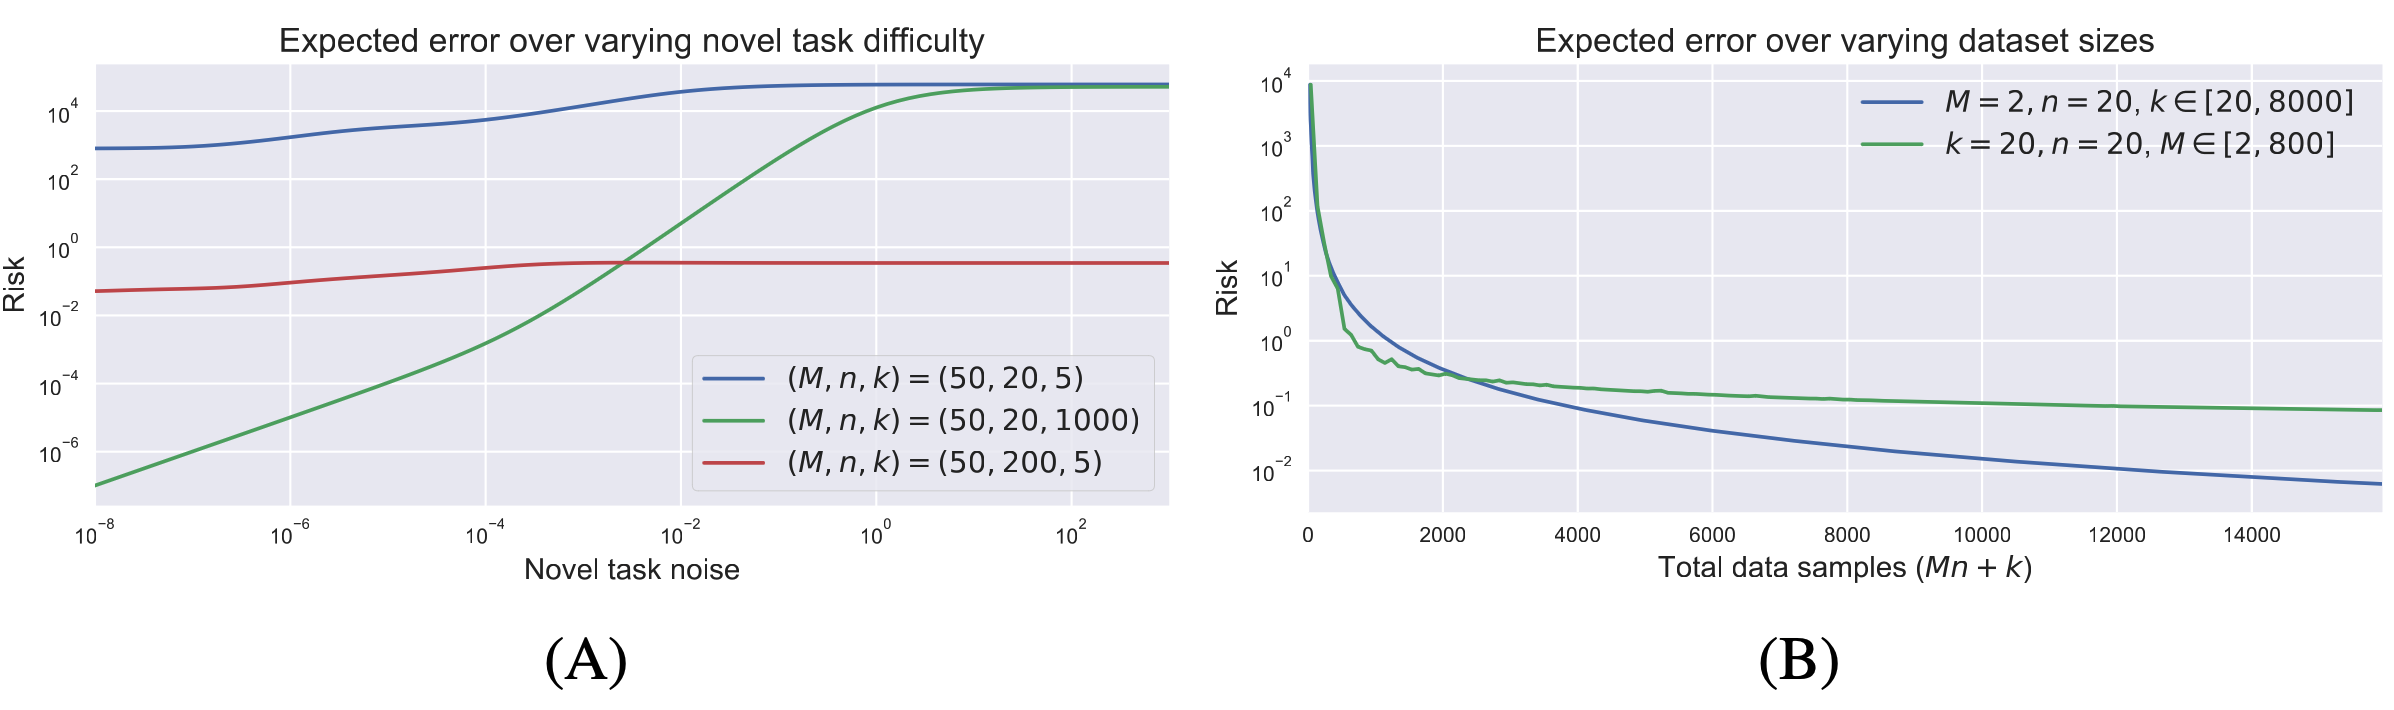
\includegraphics[width=6\linewidth]{main/images/gaussian.png}
\caption{The expected error rate of the hierarchical MAP estimator, $\thetaEst$, over different environment
hyperparameter settings. \textbf{A)} The novel task observation noise is increased, making the novel task harder to learn. \textbf{B)} We increase the size of the dataset, in one case adding new tasks ($M$) and in the other adding new novel task data samples ($k$).}
\label{fig:hierarchical_lreg_simulation}
\end{figure}
\else
\begin{figure}
\centering
\begin{minipage}{0.5\linewidth}%
    \centering%
    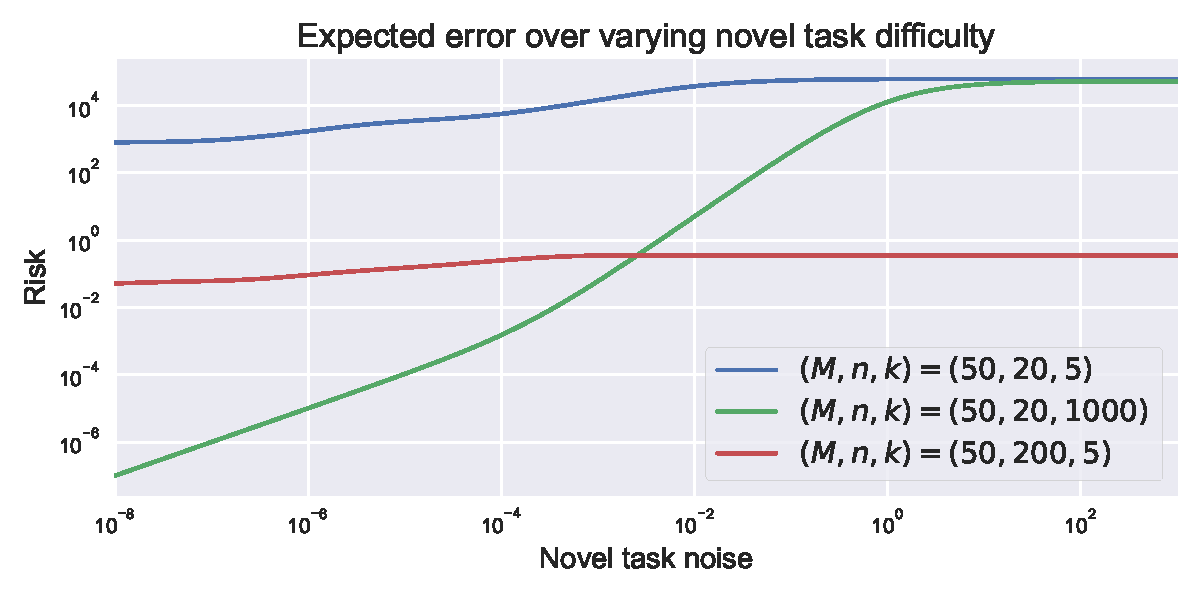
\includegraphics[width=\linewidth]{main/images/varying_task_difficulty.pdf}
    (A)
\end{minipage}%
\begin{minipage}{0.5\linewidth}%
    \centering%
    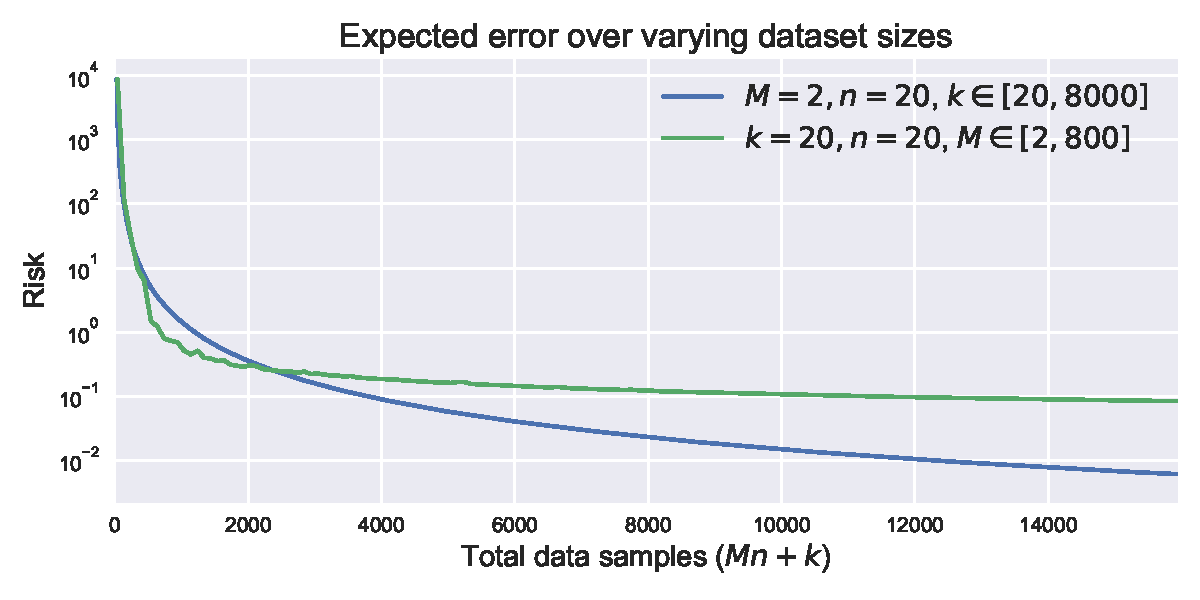
\includegraphics[width=\linewidth]{main/images/map_M_plateau.pdf}
    (B)
\end{minipage}
\caption{The expected error rate of the hierarchical MAP estimator, $\thetaEst$, over different environment
hyperparameter settings. \textbf{A)} The novel task observation noise is increased, making the novel task harder to learn. \textbf{B)} We increase the size of the dataset, in one case adding new tasks ($M$) and in the other adding new novel task data samples ($k$).}
\label{fig:hierarchical_lreg_simulation}
\end{figure}
\fi
